% This is LLNCS.DEM the demonstration file of
% the LaTeX macro package from Springer-Verlag
% for Lecture Notes in Computer Science,
% version 2.3 for LaTeX2e
%
\documentclass{llncs}
%

\usepackage{expl3}
\usepackage{hyperref}

\ExplSyntaxOn
\newcommand{\clearurl}[1]{
    \tl_set:Nn \parsed_url {#1}
    \regex_replace_all:nnN {.*:\/\/(?:www.)?(.*[^\/])\/?} {\1} \parsed_url
    \href{#1}{\texttt{\parsed_url}}
}
\ExplSyntaxOff
\usepackage{ngerman}
\usepackage[T1]{fontenc}
\usepackage[utf8]{inputenc}
\usepackage{makeidx}  % allows for indexgeneration
\usepackage{multirow}
\usepackage{rotating}
\usepackage{verbatim}
\usepackage{hyperref}
\usepackage{graphicx}
\usepackage{amssymb}   % AMS-Sonderzeichen
\usepackage{tabularx}  % Für tabularx und newcolumntype
% \usepackage[paper=a4paper,left=30mm,right=30mm,top=30mm,bottom=30mm]{geometry}
\usepackage{color}
\usepackage{ragged2e}
\usepackage{float} % 
\usepackage{ifpdf}
% \usepackage{titlesec}
\usepackage{xcolor}    % Lieber xcolor als color. Dann klappt auch das listings gut mit den Farben
\usepackage{listings}
\usepackage{upquote}   % Verändert die Ausgabe der einfachen Anführungszeichen innerhalb von verbatim
\usepackage{eurosym}   % Euro-Zeichen: \euro
\usepackage{lastpage}  % \pageref{LastPage} um die Anzahl der Seiten zu erhalten
% hiermit kann man auch umlaute copy-pasten
\usepackage{lmodern}
\selectlanguage{german}
\usepackage{fancyhdr}
\pagestyle{fancy}
%

\ifpdf
\pdfinfo{
   /Author (Fabian Matzollek, Jakub Naruszko, Louisa Bahr, Michael Nguyen, Mustafa Islek
   /Title  (Betriebssysteme und Rechnernetze -- Buzzword-Bingo-Spiel mit Interprozesskommunikation-- SS2024)
   /Subject (Betriebssysteme, Rechnernetze, Bingo, Buzzword-Bingo-Spiel, Dokumentation)
   /Keywords (Betriebssysteme, Rechnernetze, Werkstück A, SS2024, Bingo, Buzzword-Bingo-Spiel, Dokumentation)
}
\fi

\setlength{\parindent}{0pt}    % Erste Zeile eines Absatzes nicht einrücken
\parskip2ex                    % Absatzabstand
\setlength{\itemsep}{0ex plus0.2ex}
\sloppy                        % Auf jeden Fall die Seitenränder einhalten.

\newcommand{\was}{Buzzword-Bingo-Spiel Dokumentation}
\newcommand{\wer}{Buzzword-Bingo-Spiel mit Interprozesskommunikation}
\newcommand{\wann}{SS2024}

\renewcommand{\headrulewidth}{0.4pt}
\renewcommand{\footrulewidth}{0.4pt}
\lhead[\wann]{\wer}
\rhead[\wer]{\wann}
\chead[]{}
\lfoot[Seite \thepage\ von \pageref{LastPage}]{\was}
\rfoot[\was]{Seite \thepage\ von \pageref{LastPage}}
\cfoot[]{}
\pagestyle{fancy}


% Hurenkinder und Schusterjungen komplett verbieten.
\clubpenalty = 10000 
\widowpenalty = 10000 
\displaywidowpenalty = 10000
% Diese Begriffe bezeichnen den Makel beim Textsatz, wenn eine Seite mit der ersten Zeile eines Absatzes endet (so genannter Schusterjunge) oder eine neue Seite mit der letzten Zeile eines Absatzes beginnt (so genanntes Hurenkind).


% Wir definieren ein paar Farben
\definecolor{Brown}{cmyk}{0,0.81,1,0.60}
\definecolor{OliveGreen}{cmyk}{0.64,0,0.95,0.40}
\definecolor{CadetBlue}{cmyk}{0.62,0.57,0.23,0}
\definecolor{lightlightgray}{gray}{0.9}
\definecolor{FrankfurtBlue}{HTML}{3333b2}

% Hier fängt das Dokument an!
\begin{document}

%
% \frontmatter          % for the preliminaries
%
% \tableofcontents
%
\mainmatter              % start of the contributions

\title{Buzzword-Bingo-Spiel mit Interprozesskommunikation}
%
\author{Fabian Matzollek, Jakub Naruszko, Louisa Bahr, Michael Nguyen, Mustafa Islek}
%
\institute{
Frankfurt University of Applied Sciences\\
(1971-2014: Fachhochschule Frankfurt am Main)\\
Nibelungenplatz 1\\
60318 Frankfurt am Main\\
\email{FJLMMBingoSpiel@proton.me}
}

\maketitle              % typeset the title of the contribution

\begin{abstract}
Diese Dokumentation beschreibt die Entwicklung eines Buzzword-Bingo-Spiels, welches Python als Programmiersprache nutzt. Das Spiel spielt man in der Shell, mit der Möglichkeit, eigene Wörter zu wählen, das Spielfeld zu bestimmen und mehrere Spieler gleichzeitig gegeneinander antreten zu lassen. Ziel des Spiels ist es, wie beim herkömmlichen Bingo, alle Wörter in einer Zeile, Spalte oder Diagonale zu markieren und die übermäßige Verwendung von Schlagwörter, die keinen Inhalt besitzen, zu kritisieren. Außerdem verwendet das Spiel eine GUI-Bibliothek, die das Spiel übersichtlicher darstellt.

 
\end{abstract}

Das Projekt wurde im Rahmen einer Portfolioprüfung im Modul Betriebssysteme und Rechnernetze an der University of Applied Sciences in Frankfurt durchgeführt. Ziel war es, die grundlegenden Konzepte der Interprozesskommunikation und der Python-Programmierung zu erlernen und vertiefen. Die folgende Dokumentation gibt einen Überblick über die Architektur des Spiels, die verwendeten Mittel und Bibliotheken, sowie die Herausforderungen und Lösungen, die während der Entwicklung auftraten. 

\section{Die Anforderungen des Spiels}

In erster Linie soll das Spiel funktionsfähig sein, d.h. ausführbar sein und keine Fehler in der Nutzung beinhalten. Außerdem soll es folgende Funktionen besitzen: 
\begin{itemize} 
    \item Auswahl zufälliger Wörter aus einer benutzerdefinierten Wörterliste.
    \item Einfügen der Wörter in eine Matrix variabler Größe.
    \item Die Mitte des Feldes (falls vorhanden) ist ein Joker.
    \item Anzahl und Namen der Spieler sind wählbar.
    \item Kommandozeilenanwendung mit verständlich kommentiertem Code.
    \item Jeder Spieler spielt in einem eigenen Prozess auf demselben Computer.
    \item Spieler können Wörter markieren und Fehler rückgängig machen.
    \item Grafische Ausgabe erfolgt durch eine GUI-Bibliothek in der Shell.
    \item Erkennung und sinnvolle Behandlung fehlerhafter Eingaben.
    \item Sieg eines Spielers wird für alle Teilnehmer erkennbar angezeigt.
    \item Erstellung von Logdateien für jeden Spieler.
    \item Ein Spieler eröffnet die Partie, andere können beitreten.

\end{itemize}

Die Anforderungen wurden aus diesem \href{https://www.christianbaun.de/BSRN24/Skript/bsrn_SS2024_portfoliopruefung_teil_1_alternative_3.pdf}{\textbf{Dokument}}\footnote{\url{https://www.christianbaun.de/BSRN24/Skript/bsrn_SS2024_portfoliopruefung_teil_1_alternative_3.pdf}} übernommen.
 


\section{Die Aufteilung der Aufgaben}


Zu Beginn des Projekts wurden die Aufgaben klar aufgeteilt. Bei der Umsetzung dieser klaren Aufteilung entstanden jedoch Probleme. Da die Aufgaben aufeinander aufbauten, war es herausfordernd, nur seinen Teil zu erledigen. Zum Beispiel war es schwierig, eine gute GUI zu entwickeln, während die Funktionen für das Spiel nicht fertig waren. Ebenso konnte man keine Interprozesskommunikation einbauen, solange es noch kein Fundament gab. Um dieses Problem zu lösen, wurde beschlossen, dass jeder versuchte, seinen Teil zu erledigen, aber allen anderen Gruppenmitgliedern auch half. So wurde aus der klaren Einteilung ein grober Leitfaden, der die Vorgehensweise definierte.  

\section{Benötigte Bibliotheken bzw. Imports}

Damit das Spiel funktionsfähig ist, benötigt man zusätzliche Installationen und Bibliotheken (bzw. Imports), diese sind: 
\begin{itemize} 
    \item Python\footnote{https://www.python.org/downloads/} (idealerweise 3.10.12)
    \item Ubuntu (WSL\footnote{https://learn.microsoft.com/en-us/windows/wsl/install})
    \item pip\footnote{https://pypi.org/project/pip/} zur Installation von Paketen (\textit{sudo apt install python3-pip})
    \item rich-Bibliothek\footnote{https://github.com/Textualize/rich} (\textit{python3 -m pip install rich})
    \item prompt-toolkit-Bibliothek\footnote{https://github.com/prompt-toolkit/python-prompt-toolkit} (\textit{python3 -m pip install rich})

\end{itemize}

\section{Bibliotheken und Imports}

Um unnötige Imports zu vermeiden, nutzen wir als externe Bibliotheken 'rich' und 'prompt-toolkit'. Eine ausführliche Erklärung aller Imports:

\begin{itemize}
    \item \texttt{os}: Bietet eine Schnittstelle zu Betriebssystemfunktionen wie das Arbeiten mit Dateisystemen und Umgebungsvariablen.
    \item \texttt{sys}: Ermöglicht den Zugriff auf systembezogene Parameter und Funktionen, einschließlich des Beendens des Programms und des Arbeitens mit der Standard-Eingabe und -Ausgabe.
    \item \texttt{random}: Stellt Funktionen zur Verfügung, um Zufallszahlen zu generieren und zufällige Auswahlvorgänge durchzuführen.
    \item \texttt{time}: Ermöglicht den Zugriff auf zeitbezogene Funktionen wie das Messen der Zeit und das Erzeugen von Pausen.
    \item \texttt{rich}: Wird verwendet, um die Konsole zu steuern und Inhalte wie Tabellen und dekorative Panels farbig anzuzeigen.
    \item \texttt{prompt\_toolkit}: Ermöglicht das Erstellen und Verwalten von interaktiven Benutzereingaben sowie das Erstellen von Dialogen und die Formatierung von Texteingaben.
    \item \texttt{datetime}: Stellt Klassen zur Verfügung, um mit Datum und Uhrzeit zu arbeiten.
\end{itemize}

\section{Funktionen und Methoden}

In den nächsten Abschnitten werden die Funktionen und Methoden des Spiels gezeigt und erklärt. Aus Platz- und Visualisierungsgründen, werden nur, aus unserer Sicht, die wichtigsten Methoden erklärt. Ggf. werden Methoden auch verkürzt dargestellt oder so verändert, dass diese kürzer sind aber die Funktion genau die gleiche bleibt.

\subsection{Initialisierung der Wörterliste}

Die Wörter werden von einer Wörterliste geladen. Der Nutzer kann die Wörterliste selbst gestalten und bei jedem Spiel diese ändern bzw. eine neue Liste verwenden.

\lstset{
language=Python,
\renewcommand{\lstlistingname}{Code-Auschnitt},
captionpos=b,
label=code,
basicstyle=\ttfamily\footnotesize,      % Code font, Examples: \footnotesize, \ttfamily
keywordstyle=\color{FrankfurtBlue},     % Keywords font ('*' = uppercase)
commentstyle=\color{gray},              % Comments font
numbers=left,                           % Line nums position
numberstyle=\footnotesize,              % Line-numbers fonts
stepnumber=1,                           % Step between two line-numbers
numbersep=5pt,                          % How far are line-numbers from code
backgroundcolor=\color{lightlightgray}, % Choose background color
frame=trbl,                             % A frame around the code
tabsize=2,                              % Default tab size
captionpos=b,                           % Caption-position = bottom
breaklines=true,                        % Automatic line breaking?
breakatwhitespace=false,                % Automatic breaks only at whitespace?
showspaces=false,                       % Dont make spaces visible
showstringspaces=false,                 % 
showtabs=false,                         % Dont make tabs visible
columns=fixed,                          % Column format
morekeywords={},                        % Specific keywords
literate=%
{Ö}{{\"O}}1
{Ä}{{\"A}}1
{Ü}{{\"U}}1
{ö}{{\"o}}1
{ä}{{\"a}}1
{ü}{{\"u}}1
{ß}{{\ss}}1
{~}{{\textasciitilde}}1
}
\begin{lstlisting}[caption=Laden der Wörterliste]
def initialize_file(filename): 
    global buzzwords_list
    try:
        with open(filename) as file:  # Öffnet die Datei
            reader = file.readlines()  # Liest die Datei ein
            buzzwords_list = [i.strip() for i in reader]  # Entfernt Zeilenumbrüche und speichert Wörter in Liste
        random.shuffle(buzzwords_list)  # Mischt die Liste, um zufällige Auswahl zu gewährleisten
    except FileNotFoundError:
        console.print(f"Fehler: Datei '{filename}' nicht gefunden.", style="bold red")
        return False
    return True
\end{lstlisting}

Der Nutzer kann durch die Funktion \textit{get\_filename()} die Wörterliste selbst wählen, indem er den Namen der Wörterliste eingibt. Dies geschieht durch folgenden Code:




\begin{lstlisting}[caption=Auswahl der Wörterliste]
def get_filename():
    [...]
        filename = session.prompt(HTML("Geben Sie den <ansigreen>Dateinamen</ansigreen> ein, aus dem die Wörter gezogen werden sollen: ")) # Prompt zur Eingabe des Dateinamens
        if initialize_file(filename):
            return filename
\end{lstlisting}

Bei entwicklung der Wörterlisten entstanden keine Probleme. Um das Spiel einfacher zu gestalten haben, gibt es bei der vorgegebenen Wörterliste nur kurze englische Wörter. Dies vermeided viele Probleme, wie den Umgang mit deutschen Umlauten oder das Strecken der Wörterfelder
\subsection{Verwaltung von Spielern}

Bevor das Spiel beginnt, wird abgefragt, wie viele Spieler am Spiel teilnehmen. Dies geschieht durch die Funktion \textit{get\_player\_count()}, die ebenso, wie die \textit{get\_filename()}-Funktion, eine Prompt zur Eingabe nutzt. 

\begin{lstlisting}[caption=Spieleranzahl Bestimmung]
def get_player_count():
    [...]
            playercount = int(session.prompt(HTML("Geben Sie die <ansicyan>Spieleranzahl</ansicyan> ein: ")))
            return playercount
        except ValueError:
            console.print("Fehler: Die Eingabe muss eine ganze Zahl sein.", style="bold red")
\end{lstlisting}

Alle Abfragen (Wörterliste, Spieleranzahl, Spielernamen, Feldgröße) erfolgen nach dem gleichen Prinzip. Durch eine Aufforderung muss der Spieler die Werte bestimmen, bevor das Spiel starten kann. Die Besonderheit bei der def \textit{get\_player\_names()}-Funktion ist, dass diese den Wert von \textit{playercount} übernimmt.

\subsection{Die Generierung des Spielfelds}

Bevor die Karten generiert werden, muss der Spieler zunächst die Feldgröße bestimmen. Dies passiert durch zwei Funktionen \textit{get\_dimensionx} und \textit{get\_dimensiony}, die die Breite und die Länge des Felds definieren. Wie bereits beschrieben, übernimmt das Spiel die Eingabe des Spielers durch Prompts.


\begin{figure}
    \centering
    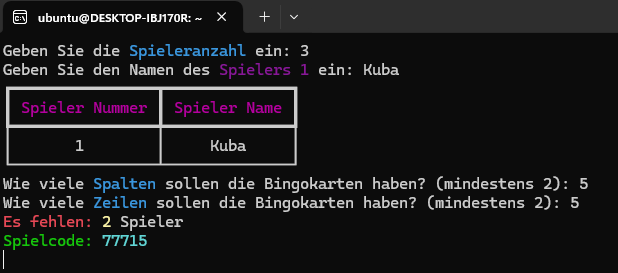
\includegraphics[width=1\linewidth]{Input.png}
    \caption{Bildschirmaufnahme des Spiels, nachdem alle Parameter eingegeben wurden}
    \label{fig:ssGame1}
\end{figure}

Nachdem alle Spieler mit dem Spielcode beigetreten sind, beginnt das Spiel, indem die Funktion \textit{generate\_bingo\_cards()} die Karten generiert. Der vollständige Code mit Kommentaren befindet sich im \textit{CA 1.7} , weswegen auf eine ausführliche Analyse hier verzichtet und stattdessen auf Probleme und Lösungen eingegangen wird.

\begin{enumerate}
\item Zu wenige Bingokarten in der Wörterliste führten zum Absturz des Spiels.
\begin{enumerate}
\item Überprüfung, ob Wörterliste größer als y*x ist, falls nicht, konkrete Fehlermeldung.
\end{enumerate}
\item Wörter kamen doppelt in dem Spielfeld eines Spielers vor.
\begin{enumerate}
\item Verwendung der Variablen 'used\_words', damit dann ein neues Wort genutzt wird.
\end{enumerate}
\item Joker befand sich nicht in der Mitte, war bei nicht korrekter Feldgröße (gerade Zahlen) vorhanden oder wurde zur Feldgröße hinzugefügt, anstatt das mittige Wort zu ersetzen. 
\begin{enumerate}
\item Korrekte Berechnung der Mitte mit '//' (abrunden), anstatt '/' (aufrunden).
\item Lösung der anderen Probleme erfolgte durch Implementierung einer if-Anweisung, bei der der Joker nur hinzugefügt wird, wenn die Feldbreite und Feldlänge nicht durch 2 teilbar ist. 
\end{enumerate}
\end{enumerate}



\subsection{Die Visualisierung}

Eine passende GUI-Bibliothek zu finden, war umständig. Da eine der Anforderung eine Kommandozeilenanwendung forderte, fielen Optionen wie tkinter\footnote{https://docs.python.org/3/library/tkinter.html} weg. Eine Alternative war pyTermTk\footnote{https://github.com/ceccopierangiolieugenio/pyTermTk}. Die Implementierung erschien aber zu aufwendig und komplex, weswegen rich\footnote{https://github.com/Textualize/rich} zum Einsatz kam.



\begin{figure}[H]
    \centering
    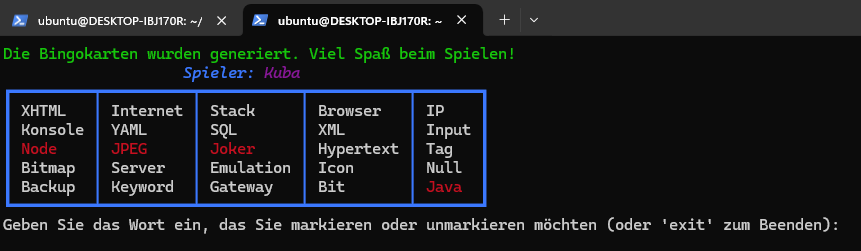
\includegraphics[width=1\linewidth]{GUI1.png}
    \caption{Das Layout des Spiels}
    \label{fig:layout1}
\end{figure}

\begin{lstlisting}[caption=Umsetzung der Tabelle in Abbildung 2.]
def display_bingo_cards(playernamelist, matrixlist, marked_words):  # Funktion, die die Bingokarten anzeigt
    print("\033c", end="", flush=True)  # Löscht die Konsole

    console.print("Die Bingokarten wurden generiert. Viel Spaß beim Spielen!", style="bold green")
    for i, matrix in enumerate(matrixlist):  # i ist der Index, matrix ist die Bingokarte

        table = Table(show_header=False, box=HEAVY_EDGE, border_style="bold blue",
                      title=f"[bold blue]Spieler:[/bold blue] [magenta]{playernamelist[i]}[/magenta]")

        for _ in range(len(matrix[0])):  # Spaltenanzahl
            table.add_column()

        for row in matrix:  # row ist eine Zeile der Bingokarte
            table.add_row(*[f"[red]{cell}[/red]" if cell in marked_words or cell == "Joker" else str(cell) for cell in row])  # Ausgabe der Bingokarte

        console.print(table)
\end{lstlisting}

Das Anzeigen des Spielfeldes und der Bingokarte erfolgt durch die Funktion \textit{display\_bingo\_cards()}. Für jeden Spieler entsteht eine Tabelle, gefüllt mit den entsprechenden Karten. Markierte Wörter und Joker erscheinen farblich hervorgehoben. Die fertigen Tabellen erscheinen schließlich in der Konsole. Die äußere Schleife iteriert über die Spieler und ihre Karten, während die inneren Schleifen die Spalten und Zeilen jeder Karte durchlaufen, um die Tabellen zu füllen.

\subsection{Die Logdatei}

Das Spiel speichert Ereignisse in individuellen Logdateien für jeden Spieler. Jede Logdatei dokumentiert das Starten des Spiels, sämtliche Aktionen und das Spielende. Dies ermöglicht eine einfache Nachverfolgung und Fehleranalyse. Die Erstellung und Verwaltung der Logdateien erfolgt durch die Funktionen \textit{create\_log\_file()} und \textit{log\_event()}. Die Funktion \textit{create\_log\_file()} generiert eine neue Logdatei mit einem Zeitstempel im Namen, während \textit{log\_event()} Ereignisse mit Zeitstempel in diese Datei schreibt.

\begin{lstlisting}[caption=Erstellung und Verwaltung der Logdatei]
def create_log_file(pid):
    timestamp = datetime.now().strftime("%Y-%m-%d-%H-%M-%S")
    filename = f"{timestamp}-bingo-Spieler{pid}.txt"
    log_files[0] = open(filename, 'w')
    log_files[0].write(f"{timestamp} Start des Spiels\n")
    return log_files[0]

def log_event(event):
    timestamp = datetime.now().strftime("%Y-%m-%d-%H-%M-%S")
    log_files[0].write(f"{timestamp} {event}\n")
\end{lstlisting}

\subsection{Kommunikation über Pipes}

Das Spiel nutzt Pipes zur Interprozesskommunikation, um Daten zwischen den einzelnen Spielerprozessen auszutauschen. Pipes ermöglichen eine effiziente und direkte Datenübertragung, die für das synchrone Spiel unerlässlich ist. Die Funktionen \textit{send()} und \textit{empfang()} verwalten das Senden und Empfangen von Nachrichten. \textit{sendfile()} und \textit{empfangfile()} übernehmen die Übertragung und den Empfang von Spieldaten.

Die Funktion \textit{send()} öffnet eine Pipe zum Schreiben und sendet eine Nachricht. Die Funktion \textit{empfang()} liest Nachrichten von den Pipes der Gegenspieler und speichert diese in einer Liste. \textit{sendfile()} überträgt Spieldaten an die Pipes der Gegner, während \textit{empfangfile()} die Daten von der eigenen Pipe empfängt und in einer Liste speichert.

\begin{lstlisting}[caption=Nachricht an Pipe senden]
def send(pipe, pipm):
    fifo = os.open(str(pipe), os.O_WRONLY)  # Pipe öffnen zum Schreiben
    s = f"{pipm}\n".encode()
    os.write(fifo, s)  # Pipe-Nachricht schreiben
    os.close(fifo)  # Pipe schließen
\end{lstlisting}


\section{Schlusswort}

Diese Dokumentation beschreibt die Entwicklung eines Buzzword-Bingo-Spiels, welches in Python programmiert und über die Kommandozeile ausgeführt wird. Ziel des Projekts war es, die grundlegenden Konzepte der Interprozesskommunikation und der Python-Programmierung zu erlernen und praktisch umzusetzen.

Das Spiel erlaubt es den Nutzern, eigene Wörterlisten zu verwenden, die Spielfeldgröße zu bestimmen und mehrere Spieler gleichzeitig gegeneinander antreten zu lassen. Eine benutzerfreundliche GUI-Bibliothek, \textit{rich}, wurde eingesetzt, um eine ansprechende visuelle Darstellung in der Kommandozeile zu ermöglichen. Die Funktion \textit{display\_bingo\_cards()} visualisiert die Spielkarten farbenfroh und übersichtlich, was die Benutzererfahrung erheblich verbessert.

Die Implementierung der Logdateien durch \textit{create\_log\_file()} und \textit{log\_event()} ermöglicht eine umfassende Nachverfolgung und Fehleranalyse des Spielverlaufs. Jede Aktion der Spieler wird detailliert in individuellen Logdateien dokumentiert, was besonders nützlich für Debugging-Zwecke und die Auswertung des Spielverhaltens ist.

Ein zentraler Aspekt des Spiels ist die Interprozesskommunikation mittels Pipes. Funktionen wie \textit{send()} und \textit{empfang()} gewährleisten einen reibungslosen Datenaustausch zwischen den Spielerprozessen. Trotz der robusten Implementierung gibt es Potenzial für weitere Optimierungen, insbesondere in Bezug auf die Effizienz und die Geschwindigkeit der Kommunikation. Die aktuelle Implementierung kann bei größeren Spielerzahlen zu Verzögerungen führen, weshalb ein zukünftiger Ansatz die Nutzung von Message Queues oder Sockets in Betracht ziehen könnte.

Zusammenfassend lässt sich sagen, dass das Projekt erfolgreich die Ziele der Portfolioprüfung erfüllt hat. Die entwickelten Funktionen arbeiten zuverlässig und bieten eine solide Basis für zukünftige Erweiterungen und Verbesserungen. Zu den möglichen Erweiterungen gehören die Implementierung einer grafischen Benutzeroberfläche, die Integration von Netzwerkfähigkeit für das Spielen über verschiedene Geräte hinweg und die Optimierung der Interprozesskommunikation. Diese Verbesserungen könnten die Benutzerfreundlichkeit weiter erhöhen und das Spiel auf ein neues Niveau heben.

\section{Anhang}

\begin{lstlisting}[caption=Generierung der Bingokarten]
    def generate_bingo_cards(playernamelist, xsize, ysize):  # Funktion, die die Bingokarten generiert
    matrixlist = []  # Liste der Bingokarten
    middle_x = xsize // 2  # Mitte der x-Achse zur Bestimmung des Jokers
    middle_y = ysize // 2  # Mitte der y-Achse zur Bestimmung des Jokers

    for k in playernamelist:  # Schleife, die die Bingokarten für jeden Spieler generiert
        if len(buzzwords_list) < xsize * ysize:  # Überprüfung, ob genug Buzzwörter vorhanden sind
            raise ValueError(
                "Nicht genug Buzzwords, um die Bingokarten zu füllen")  # Fehlermeldung, wenn nicht genug Buzzwörter vorhanden sind
        used_words = set()  # Set für verwendete Wörter
        matrix = []  # Liste für die Bingokarte
        for l in range(ysize):  # Zeilen
            b = []  # Liste für die Zeile
            for j in range(xsize):  # Spalten
                if xsize % 2 != 0 and ysize % 2 != 0 and l == middle_y and j == middle_x:  # Joker in der Mitte, nur wenn xsize und ysize ungerade sind
                    b.append("Joker")  # Fügt den Joker in die Mitte der Bingokarte ein
                else:
                    while True:
                        random_word = buzzwords_list.pop(0)  # Nimmt das erste Element aus der Liste und entfernt es, damit kein Wort doppelt vorkommt
                        if random_word not in used_words:  # Überprüfung, ob das Wort bereits verwendet wurde
                            used_words.add(random_word)  # Fügt das Wort zu den verwendeten Wörtern hinzu
                            b.append(random_word)  # Fügt das zufällige Wort in die Bingokarte ein
                            break  # Beendet die Schleife, wenn ein neues Wort gefunden wurde
                    buzzwords_list.append(random_word)  # Füge das Wort zurück zur Liste, damit es nicht verloren geht
            matrix.append(b)  # Fügt die Zeile der Bingokarte in die Bingokarte ein
        matrixlist.append(matrix)  # Fügt die Bingokartenmatrix einer Person in die Bingokartenliste ein
    return matrixlist  # Gibt die Liste der Bingokarten zurück

\end{lstlisting}




\end{document}
